% задание и сама лабораторная работа
\newpage
\section*{Задание}
\addcontentsline{toc}{section}{\tocsecindent{Задание}}
\Large{Лабораторная работа №2}

\begin{enumerate}
	\item Используя только функции car и cdr, написать выражения, возвращающие:
	\begin{itemize}
		\item второй $=$ cadr
		\item третий $=$ caddr
		\item четвертый элементы заданного списка $=$ cadddr
	\end{itemize}
	\item Что будет в результате вычисления выражений:\\
	\begin{minipage}[t]{1.1\textwidth}
		\centering\raisebox{\dimexpr \topskip-\height}{%
		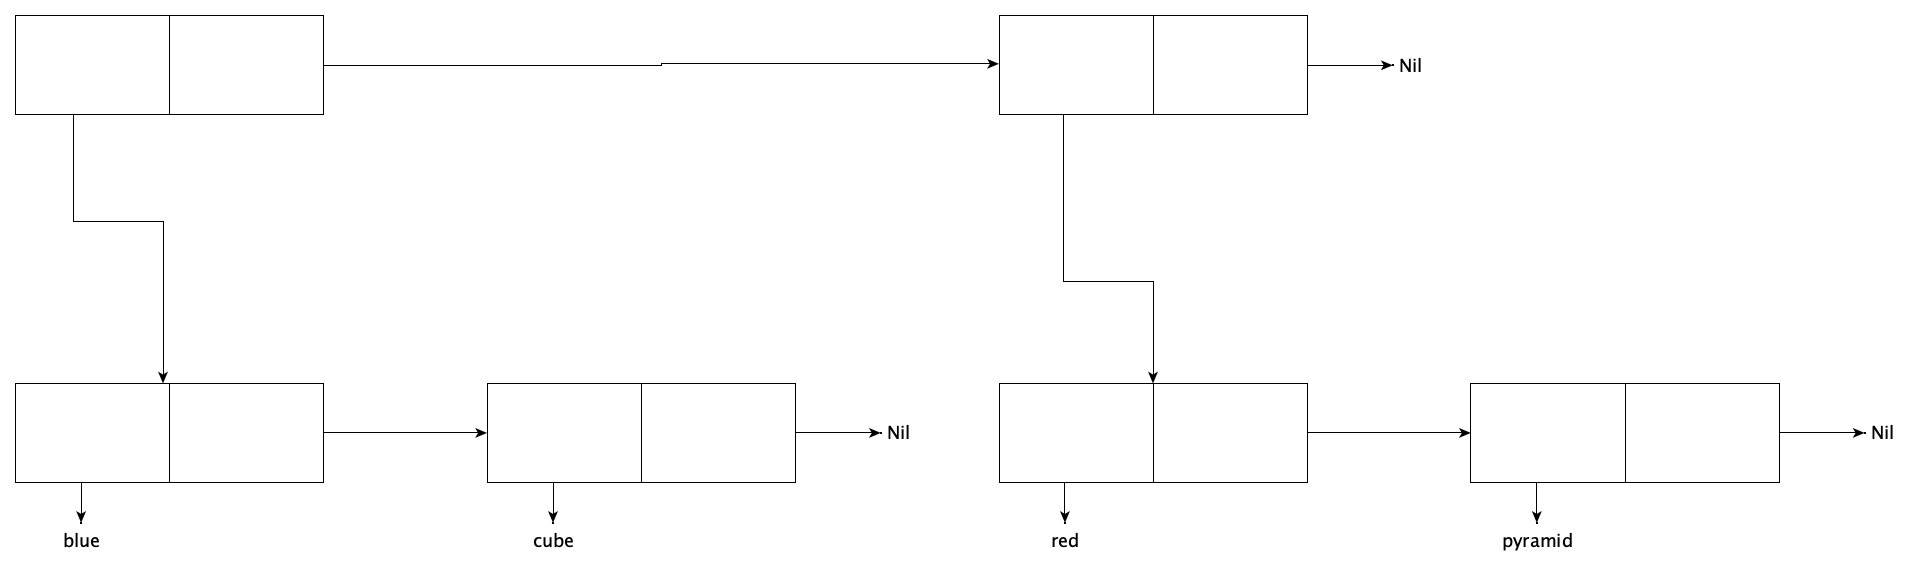
\includegraphics[width=\textwidth]{1.png}}
		\captionof{figure}{'((blue cube) (red pyramid))}
		\label{fig1}
	\end{minipage}\hfill
	\\
	\begin{minipage}[t]{1.1\textwidth}
		\centering\raisebox{\dimexpr \topskip-\height}{%
		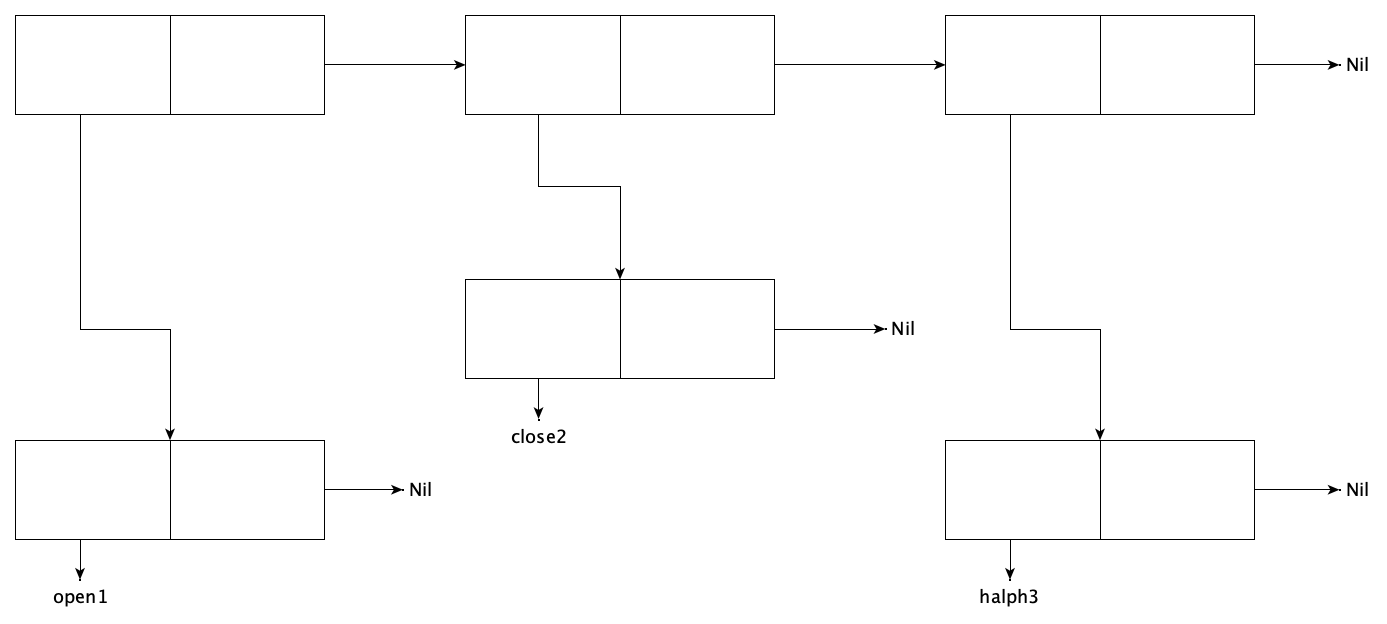
\includegraphics[width=\textwidth]{2.png}}
		\captionof{figure}{'((abc) (def) (ghi))}
		\label{fig2}
	\end{minipage}\hfill
	\begin{itemize}
		\item (caadr '((blue cube) (red pyramid))) $=$ red
		\item (cdar '((abc) (def) (ghi))) $=$ Nil
		\item (cadr '((abc) (def) (ghi))) $=$ (def)
		\item (caddr '((abc) (def) (ghi))) $=$ (ghi)
	\end{itemize}
\end{enumerate}